\section{Marco Teórico}

Este capítulo establece los fundamentos científicos y matemáticos del sistema propuesto. Se aborda desde la psicología cognitiva de la memoria hasta el álgebra lineal aplicada al procesamiento de lenguaje natural, proporcionando una base rigurosa pero accesible para entender la integración entre retención (UIR) y comprensión (UIC).

\subsection{Memoria Humana y la Curva del Olvido}

\subsubsection{Definición y Concepto}
La memoria humana no es un almacén estático de información, sino un proceso dinámico de codificación, almacenamiento y recuperación. Un hallazgo fundamental en la psicología cognitiva es que el olvido no es un fallo del sistema, sino una característica intrínseca: olvidamos para no saturarnos, y el ritmo al que olvidamos sigue patrones matemáticos predecibles.

\begin{tcolorbox}[colback=green!5!white,colframe=green!75!black,title=Analogía de Feynman: El Sendero en el Bosque]
Imagina que tu cerebro es un bosque denso. Aprender algo nuevo es como caminar por primera vez entre la maleza: dejas un rastro apenas visible.
\begin{itemize}
    \item Si no vuelves a pasar por ahí, la maleza crece y el camino desaparece (olvido).
    \item Si caminas por ese sendero repetidamente, la tierra se aplana, la maleza se aparta y se convierte en un camino claro y fácil de transitar (consolidación).
    \item Cuanto más tiempo pasa sin que lo uses, más difícil es volver a encontrarlo.
\end{itemize}
La \textbf{fuerza de la memoria} es qué tan marcado está ese camino.
\end{tcolorbox}

\subsubsection{Fundamento Matemático (Ebbinghaus)}
Hermann Ebbinghaus, en 1885, fue el primero en cuantificar este fenómeno. A través de experimentos rigurosos consigo mismo memorizando sílabas sin sentido, descubrió la \textbf{Curva del Olvido}.

La probabilidad de recordar una información $R$ en un tiempo $t$ decae exponencialmente:

\begin{equation}
R(t) = e^{-\frac{t}{S}}
\end{equation}

Donde:
\begin{itemize}
    \item $R(t) \in [0,1]$: Retención (probabilidad de recuerdo).
    \item $t$: Tiempo transcurrido desde el último repaso.
    \item $S$: \textbf{Estabilidad de la memoria} (fuerza del recuerdo).
\end{itemize}

\begin{figure}[h]
\centering
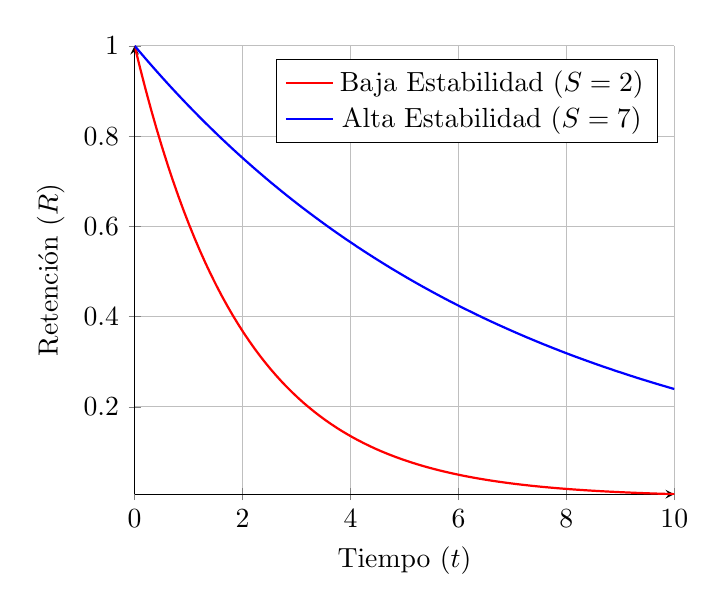
\begin{tikzpicture}
    \begin{axis}[
        xlabel={Tiempo ($t$)},
        ylabel={Retención ($R$)},
        domain=0:10,
        samples=100,
        axis lines=left,
        legend pos=north east,
        grid=major
    ]
    \addplot[color=red, thick] {exp(-x/2)};
    \addlegendentry{Baja Estabilidad ($S=2$)}
    
    \addplot[color=blue, thick] {exp(-x/7)};
    \addlegendentry{Alta Estabilidad ($S=7$)}
    \end{axis}
\end{tikzpicture}
\caption{Comparación de curvas de olvido. Una mayor estabilidad $S$ (curva azul) implica una caída más lenta de la retención.}
\end{figure}

\textbf{¿Por qué exponencial?}
En la naturaleza, muchos procesos de decaimiento son exponenciales (desintegración radiactiva, enfriamiento de un café). Esto ocurre cuando la tasa de pérdida es proporcional a la cantidad actual. En la memoria, cuanto más fresco está el recuerdo, más rápido se desvanece inicialmente, estabilizándose con el tiempo.

\subsubsection{Implementación en Nuestro Trabajo}
En nuestro sistema, utilizamos esta formulación para derivar la UIR. Asumimos que cada tarjeta tiene su propia curva de olvido, caracterizada por su estabilidad $S$ (que nosotros llamamos UIR).
\textit{Ver implementación en \texttt{app.py}, función \texttt{compute\_uir}.}

\subsection{Modelos de Repetición Espaciada (SRS)}

\subsubsection{El Algoritmo SM-2 de Anki}
Los sistemas de repetición espaciada (SRS) buscan optimizar $t$ (cuándo repasar) para maximizar $S$ (estabilidad) con el mínimo esfuerzo. El algoritmo más famoso es el SM-2, utilizado por Anki.

\textbf{Funcionamiento Simplificado:}
El algoritmo determina el próximo intervalo $I$ basándose en:
1.  El intervalo previo ($I_{prev}$).
2.  Un factor de facilidad ($EF$), que indica qué tan difícil es la tarjeta.
3.  La calidad de la respuesta ($q$) dada por el usuario (0-3).

\textbf{Matemática del Algoritmo:}
Si la respuesta es correcta ($q \ge 2$):

\begin{equation}
I_{n} = I_{n-1} \times EF
\end{equation}

El Factor de Facilidad ($EF$) se actualiza en cada repaso para adaptarse al usuario:

\begin{equation}
EF_{new} = EF_{old} + (0.1 - (3-q) \cdot (0.08 + (3-q) \cdot 0.02))
\end{equation}

\textbf{Análisis Computacional:}
El SM-2 es un algoritmo \textit{greedy} (avaro): toma decisiones locales óptimas basadas solo en el historial de esa tarjeta específica. No considera el contexto ni las relaciones entre conceptos.
\textit{Ver implementación en \texttt{app.py}, función \texttt{compute\_anki\_interval\_pure}.}

\subsection{Diferencia entre Recuerdo y Comprensión}

Es crucial distinguir dos procesos cognitivos que a menudo se confunden:

\begin{enumerate}
    \item \textbf{Recuerdo (Retention):} Es la capacidad de recuperar un dato específico. Es binario (lo sabes o no) y atómico.
    \item \textbf{Comprensión (Comprehension):} Es la capacidad de conectar ese dato con otros, entender su causa, efecto y contexto. Es relacional y estructural.
\end{enumerate}

\begin{tcolorbox}[colback=blue!5!white,colframe=blue!75!black,title=Ejemplo Didáctico]
\textbf{Recuerdo:} Memorizar que "La capital de Francia es París". Puedes repetirlo como un loro sin saber qué es Francia o qué es una capital.
\textbf{Comprensión:} Entender que París es el centro político y económico de Francia, situado en el río Sena, y cómo su historia influyó en la Revolución Francesa.
\end{tcolorbox}

\textbf{En nuestro modelo:}
\begin{itemize}
    \item \textbf{UIR} mide el Recuerdo (fuerza de la huella de memoria individual).
    \item \textbf{UIC} mide la Comprensión (densidad de conexiones con otros conocimientos).
\end{itemize}

\subsection{Embeddings y Representación Vectorial del Lenguaje}

Para que una computadora "entienda" el significado de las palabras y pueda medir la comprensión, necesitamos traducir el lenguaje humano a matemáticas.

\subsubsection{¿Qué es un Vector en este contexto?}
Un vector no es más que una lista ordenada de números que representa un punto en un espacio multidimensional. En nuestro caso, cada dimensión del espacio corresponde a una palabra o concepto posible.

\begin{tcolorbox}[colback=yellow!5!white,colframe=yellow!75!black,title=Analogía de Feynman: Coordenadas de Significado]
Imagina un mapa gigante de conceptos.
\begin{itemize}
    \item Cada palabra tiene una "dirección" (coordenadas GPS).
    \item La palabra "Rey" está en la coordenada [10, 50].
    \item La palabra "Reina" está en [12, 48]. Están muy cerca.
    \item La palabra "Manzana" está en [90, 5]. Está muy lejos.
\end{itemize}
Los embeddings son simplemente esas coordenadas.
\end{tcolorbox}

\subsubsection{Normalización: Volumen vs. Dirección}
Un concepto clave es la \textbf{normalización}. A veces, una frase puede tener vectores con números muy grandes simplemente porque es más larga o repite palabras.

\textbf{Analogía:} Imagina dos personas señalando hacia la luna.
\begin{itemize}
    \item La persona A grita: "¡Allí está la luna!".
    \item La persona B susurra: "Allí".
\end{itemize}
Ambos señalan en la \textbf{misma dirección} (mismo significado), pero con diferente "fuerza" (magnitud). Al normalizar los vectores (dividirlos por su longitud), hacemos que ambos tengan longitud 1. Así, solo comparamos hacia dónde apuntan, ignorando si gritan o susurran.

\subsubsection{Técnica Usada: TF-IDF}
En nuestra implementación, usamos TF-IDF (Term Frequency - Inverse Document Frequency).
\begin{itemize}
    \item \textbf{TF (Frecuencia):} ¿Cuántas veces aparece la palabra "célula" en esta tarjeta? (Si aparece mucho, es importante).
    \item \textbf{IDF (Frecuencia Inversa):} ¿Cuántas veces aparece "célula" en \textit{todas} las tarjetas? (Si aparece en todas, es una palabra común y pierde importancia distintiva).
\end{itemize}

Esto genera un vector para cada tarjeta donde cada dimensión representa la importancia de una palabra específica.
\textit{Ver implementación en \texttt{app.py}, uso de \texttt{TfidfVectorizer}.}

\subsection{Matrices de Similitud y Grafos Semánticos}

Aquí es donde aplicamos álgebra lineal para modelar la "Comprensión" (UIC). Queremos saber qué tan relacionada está la tarjeta A con la tarjeta B.

\subsubsection{El Producto Punto y la Similitud Coseno}
Para comparar dos vectores (dos tarjetas), usamos la \textbf{Similitud Coseno}.

\begin{figure}[h]
\centering
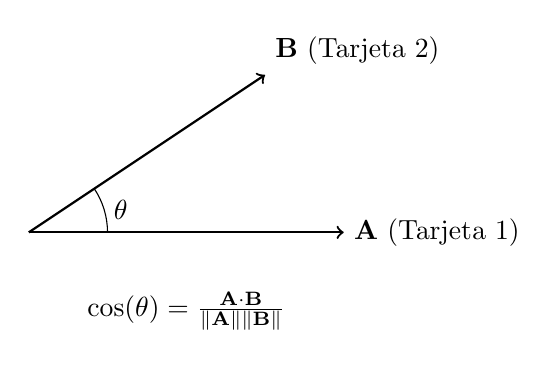
\begin{tikzpicture}
    \draw[->, thick] (0,0) -- (4,0) node[right] {$\mathbf{A}$ (Tarjeta 1)};
    \draw[->, thick] (0,0) -- (3,2) node[above right] {$\mathbf{B}$ (Tarjeta 2)};
    \draw (1,0) arc (0:33.69:1) node[midway, right] {$\theta$};
    \node at (2,-1) {$\cos(\theta) = \frac{\mathbf{A} \cdot \mathbf{B}}{\|\mathbf{A}\| \|\mathbf{B}\|}$};
\end{tikzpicture}
\caption{Representación geométrica de la similitud coseno. El ángulo $\theta$ determina la similitud semántica.}
\end{figure}

\textbf{Paso a paso para principiantes:}
1.  Tenemos dos vectores, $\mathbf{A}$ y $\mathbf{B}$.
2.  Queremos saber si apuntan a la misma dirección (significado similar).
3.  El \textbf{Producto Punto} ($\mathbf{A} \cdot \mathbf{B}$) nos dice cuánto se alinean, pero se ve afectado si un vector es más largo (tiene más palabras).
4.  Para corregir esto, dividimos por la \textbf{Magnitud} (longitud) de los vectores ($\|\mathbf{A}\|$ y $\|\mathbf{B}\|$). Esto normaliza los vectores a longitud 1.

\subsubsection{Ejemplo Numérico "De Juguete"}
Vamos a calcular la similitud entre dos frases simplificadas. Supongamos un vocabulario de solo 3 palabras: [Sol, Brilla, Quema].

\textbf{Frase A:} "El Sol brilla" $\rightarrow$ Vector $\mathbf{A} = [1, 1, 0]$ (Tiene Sol, tiene Brilla, no tiene Quema).
\textbf{Frase B:} "El Sol quema" $\rightarrow$ Vector $\mathbf{B} = [1, 0, 1]$ (Tiene Sol, no tiene Brilla, tiene Quema).

\textbf{Paso 1: Producto Punto ($\mathbf{A} \cdot \mathbf{B}$)}
Multiplicamos componente a componente y sumamos:
$$ (1 \times 1) + (1 \times 0) + (0 \times 1) = 1 + 0 + 0 = 1 $$

\textbf{Paso 2: Magnitudes ($\|\mathbf{A}\|$ y $\|\mathbf{B}\|$)}
Calculamos la longitud (raíz cuadrada de la suma de cuadrados):
$$ \|\mathbf{A}\| = \sqrt{1^2 + 1^2 + 0^2} = \sqrt{2} \approx 1.414 $$
$$ \|\mathbf{B}\| = \sqrt{1^2 + 0^2 + 1^2} = \sqrt{2} \approx 1.414 $$

\textbf{Paso 3: Similitud Coseno}
$$ \text{Similitud} = \frac{1}{1.414 \times 1.414} = \frac{1}{2} = 0.5 $$

\textbf{Conclusión:} Las frases tienen una similitud del 50\%. Comparten la palabra "Sol" pero difieren en la acción.

\subsubsection{Algoritmo de Vecinos Más Cercanos (k-NN)}
Una vez tenemos la matriz de similitud completa, no nos interesa el promedio global (que suele ser muy bajo porque la mayoría de cosas no se parecen entre sí). Nos interesa el \textbf{contexto local}.

\textbf{¿Por qué k-NN?}
Imagina que quieres saber si una persona es "deportista".
\begin{itemize}
    \item \textbf{Promedio Global:} Si la comparas con toda la población mundial, la similitud es baja.
    \item \textbf{Vecinos (k-NN):} Si miras a sus 5 amigos más cercanos y todos son atletas, es muy probable que esa persona también lo sea.
\end{itemize}

En nuestro sistema, para calcular la UIC de una tarjeta, miramos sus 5 tarjetas más similares (sus "vecinos"). Si esos vecinos están muy conectados entre sí, significa que la tarjeta pertenece a un \textbf{cluster de conocimiento denso} (un tema que dominas bien).

\subsection{Estabilidad del Recuerdo y Formulaciones Logarítmicas (UIR)}

La Unidad Internacional de Retención (UIR) no es un número arbitrario; se deriva directamente de invertir la curva de Ebbinghaus.

Queremos encontrar $S$ (la estabilidad en días). Partimos de:
$$ R = e^{-\frac{t}{S}} $$

Tomamos logaritmo natural ($\ln$) a ambos lados para "bajar" el exponente (linealizar):
$$ \ln(R) = -\frac{t}{S} $$

Despejamos $S$:
\begin{equation}
S = -\frac{t}{\ln(R)}
\end{equation}

Esta $S$ es nuestra \textbf{UIR}.

\subsubsection{El Problema del Cero y el Suavizado de Laplace}
Matemáticamente, si $R=1$ (recuerdo perfecto), $\ln(1)=0$, y dividir por cero es imposible ($S \to \infty$). Si $R=0$ (olvido total), $\ln(0) = -\infty$.

Para evitar que el sistema colapse con valores extremos, usamos el \textbf{Suavizado de Laplace}.
La idea es "fingir" que siempre hemos visto al menos un éxito y un fallo antes de empezar. Es como el principio de "inocente hasta que se demuestre lo contrario".

En lugar de usar la probabilidad cruda $P = \frac{\text{éxitos}}{\text{total}}$, usamos:
\begin{equation}
P_{suavizada} = \frac{\text{éxitos} + 1}{\text{total} + 2}
\end{equation}

Esto asegura que la probabilidad nunca sea exactamente 0 ni 1, manteniendo las matemáticas estables y los intervalos dentro de rangos humanos.

\subsection{Integración entre Retención y Comprensión: UIR Efectiva}

La innovación central de nuestro modelo es que la retención no es aislada. \textbf{Entender ayuda a recordar}.

Definimos la \textbf{UIR Efectiva} ($U_{eff}$) como la UIR base modulada por la comprensión (UIC):

\begin{equation}
U_{eff} = U_{base} \cdot (1 + \alpha \cdot UIC_{local})
\end{equation}

\textbf{El Porqué Matemático:}
Estamos modelando una interacción sinérgica. El término $(1 + \alpha \cdot UIC)$ actúa como un multiplicador escalar.
\begin{itemize}
    \item Si $UIC = 0$ (sin conexiones), $U_{eff} = U_{base}$. El sistema se comporta como Anki normal.
    \item Si $UIC > 0$, la estabilidad \textit{aumenta}. Matemáticamente, estamos diciendo que la tasa de decaimiento del olvido se ralentiza gracias a la red de soporte semántico.
\end{itemize}

\subsection{Parámetros de la UIR y su Nivelación}

El modelo utiliza cuatro hiperparámetros fundamentales que controlan la dinámica del sistema. Estos no son aleatorios, sino que provienen de un análisis de estabilidad de sistemas dinámicos (ver sección de modelo propuesto).

\begin{enumerate}
    \item \textbf{$\alpha$ (Alpha) - Peso Semántico (0.2):}
    Controla cuánto influye la comprensión en la retención. Un valor de 0.2 significa que una comprensión perfecta puede mejorar la retención hasta un 20\%.
    \textit{Justificación:} Evita que la comprensión domine sobre el repaso activo.

    \item \textbf{$\gamma$ (Gamma) - Tasa de Refuerzo (0.1):}
    Cuánto aumenta la conexión semántica (UIC) tras un repaso exitoso.
    \textit{Justificación:} El aprendizaje es gradual; no conectas todo de golpe.

    \item \textbf{$\delta$ (Delta) - Tasa de Decaimiento (0.05):}
    Cuánto se debilita la conexión si fallas.
    \textit{Justificación:} $\gamma > \delta$ (2:1) asegura que es más fácil construir conocimiento que destruirlo, favoreciendo la plasticidad positiva.

    \item \textbf{$\eta$ (Eta) - Tasa de Aprendizaje UIR (0.5):}
    Cuánto crece la estabilidad base ($U_{base}$) en cada éxito.
    \textit{Justificación:} Permite que la UIR escale rápidamente en las primeras fases de aprendizaje (fase exponencial de la curva de aprendizaje).
\end{enumerate}

Estos parámetros se calibran para mantener el sistema en un equilibrio estable, evitando que los intervalos de repaso exploten hacia el infinito o colapsen a cero.
